\section{Detailed Design}
\subsection{Our design}
\subsubsection{Class diagram}

\begin{figure}[H]
 \centering
 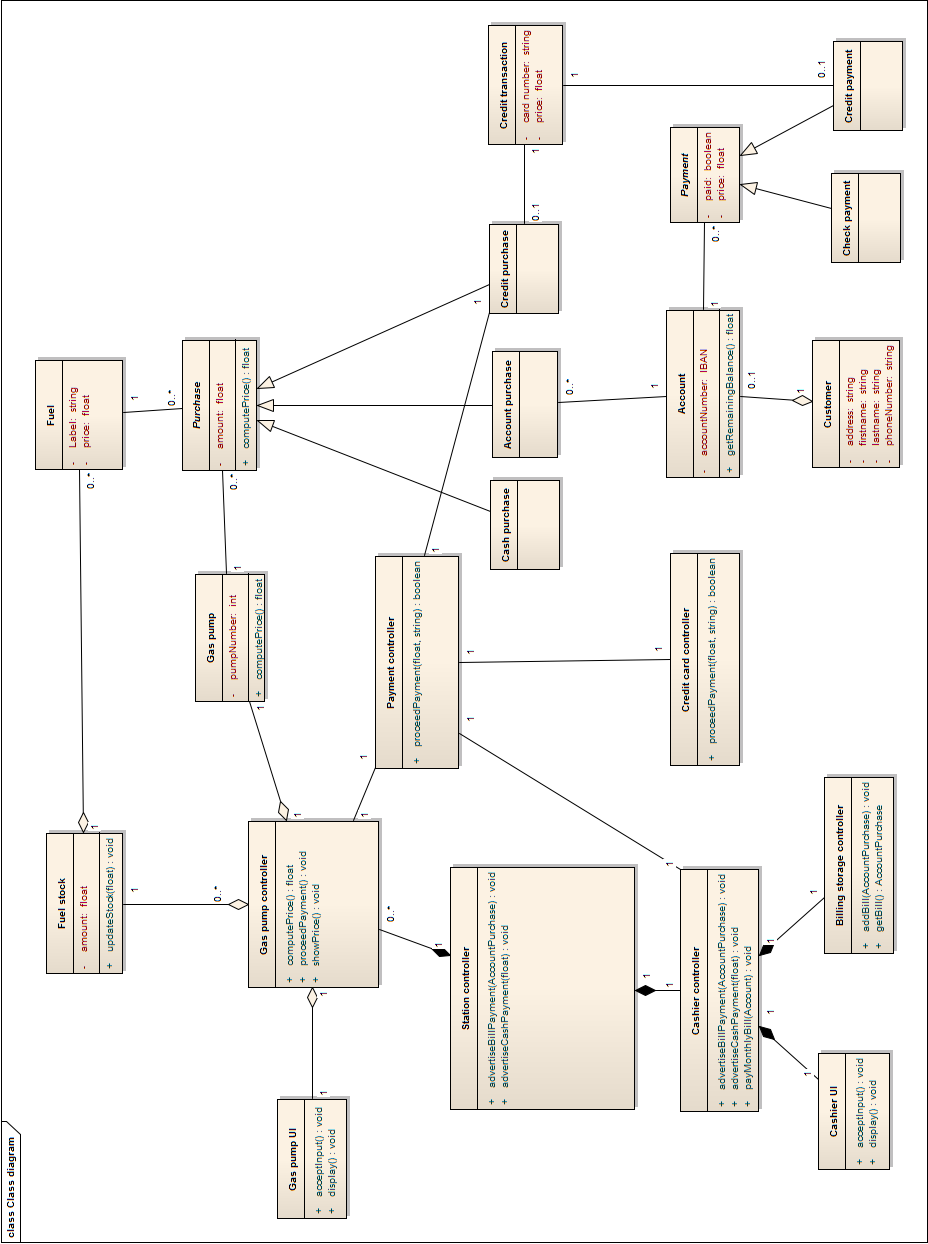
\includegraphics[width=\textwidth]{../ClassDiagram.png}
\end{figure}

\subsubsection{Description of classes}
\todo[inline]{Tanguy TODO}


\subsubsection{Uses diagram}

\begin{figure}[H]
 \centering
 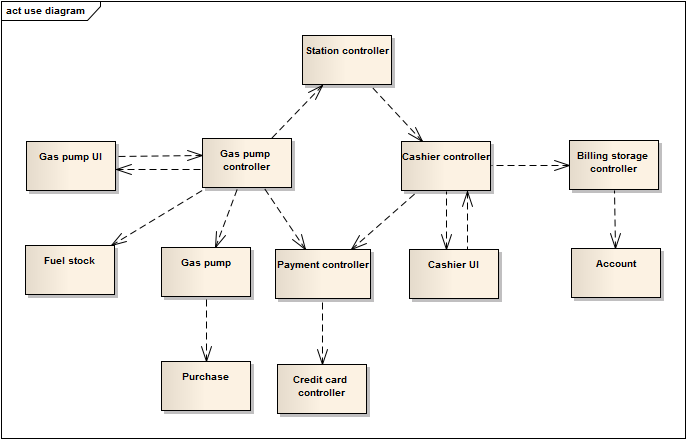
\includegraphics[width=\textwidth]{../useDiagram.png}
\end{figure}
There are 2 loops in this Uses diagram:
\begin{itemize}
	\item between \textit{Gas pump UI} and \textit{Gas pump controller}
	\item between \textit{Cashier UI} and \textit{Cashier controller}
\end{itemize}
But this is not really a problem because there are just between a view and its controller. It makes senses that the controller uses the view to update it and that the view uses the controller to notify it when an user's action occurs. We think that they can no be eliminated.


\subsection{Design Patterns}
The skeletons are written in Java.

\subsubsection{Template Method}
\begin{figure}[H]
 \centering
 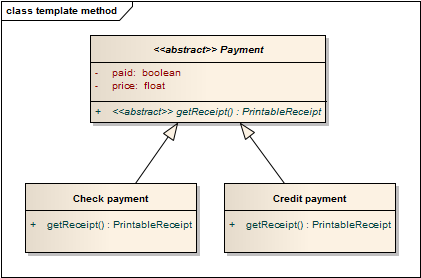
\includegraphics[width=0.75\textwidth]{../templateMethod.png}
\end{figure}

\lstinputlisting[language=java, inputencoding=utf8]{../templateMethod.java}

\subsubsection{Strategy Pattern}
\begin{figure}[H]
 \centering
 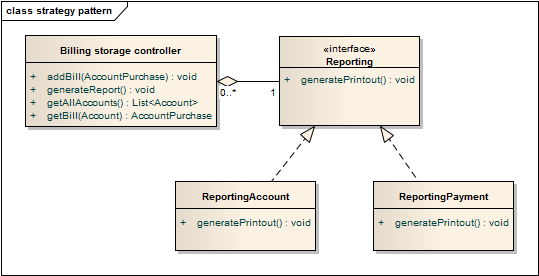
\includegraphics[width=0.8\textwidth]{../strategyPattern.png}
\end{figure}

\lstinputlisting[language=java, inputencoding=utf8]{../strategyPattern.java}


\subsubsection{Decorator Pattern}
\begin{figure}[H]
 \centering
 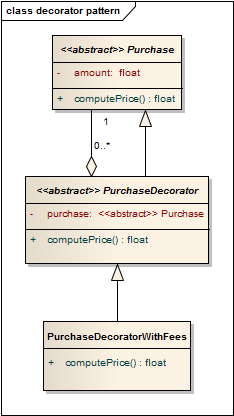
\includegraphics[width=0.35\textwidth]{../decoratorPattern.png}
\end{figure}

\lstinputlisting[language=java, inputencoding=utf8]{../decoratorPattern.java}


\subsubsection{Observer Pattern}
\begin{figure}[H]
 \centering
 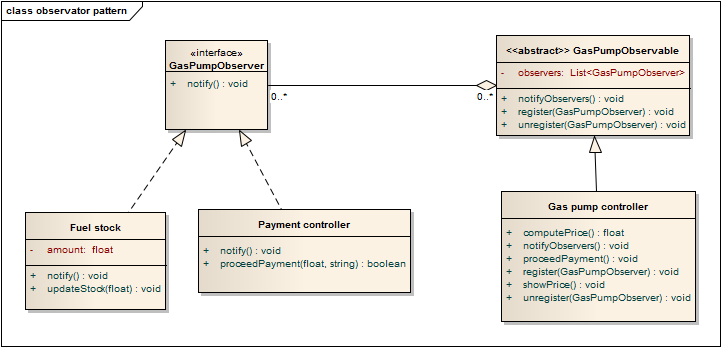
\includegraphics[width=0.9\textwidth]{../observatorPattern.png}
\end{figure}

\lstinputlisting[language=java, inputencoding=utf8]{../observatorPattern.java}


\subsubsection{Composite Pattern}
\begin{figure}[H]
 \centering
 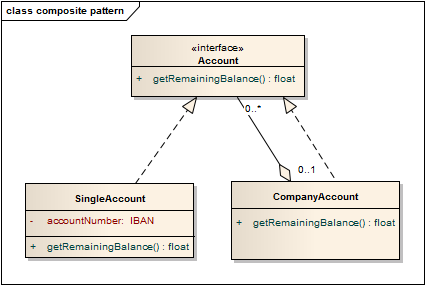
\includegraphics[width=0.8\textwidth]{../compositePattern.png}
\end{figure}

\lstinputlisting[language=java, inputencoding=utf8]{../compositePattern.java}

We can see in the snippet of code above where the new methods are implemented.
But the existing methods (the getters and setters for the bank account in this case) are implemented in the SingleAccount class. If we had other pre-existing methods in the Account, they would be implemented in the new SingleAccount class and also in the CompanyAccount. To call those methods, the developer should have a reference to the concrete object, not the new Account interface (because it does not define other methods than \textit{getRemainingBalance()}.